\documentclass[10pt]{beamer}

\usetheme[progressbar=frametitle]{metropolis}
\usepackage{appendixnumberbeamer}

\usepackage{booktabs}
\usepackage[scale=2]{ccicons}

\usepackage{pgfplots}
\usepgfplotslibrary{dateplot}

\graphicspath{{figures/}}
\usepackage{subcaption}
\usepackage{algorithm}
\usepackage[noend]{algpseudocode}
% \usepackage[font=small,labelfont=bf,tableposition=top]{caption}

\usepackage{tcolorbox}

\usepackage{xspace}
\newcommand{\themename}{\textbf{\textsc{metropolis}}\xspace}

\usefonttheme{serif} % default family is serif

\definecolor{Red}{RGB}{227,0,27}
\definecolor{Orange}{RGB}{230,159,0}
\definecolor{Black}{RGB}{0,0,0}
\definecolor{Grey}{HTML}{595959}
%\definecolor{LightGrey}{RGB}{216,216,216}
\definecolor{LightGrey}{RGB}{240,240,240}
\definecolor{White}{RGB}{255,255,255}
\setbeamercolor{title}{fg=Black}
\setbeamercolor{progress bar}{fg=Red}
\setbeamercolor{progress bar in head/foot}{fg=Orange}
\setbeamercolor{normal text}{fg=Grey}
\setbeamercolor{frametitle}{fg=Black, bg=LightGrey}
\setbeamercolor{background canvas}{bg=White}



\title{A High Performance Implementation of the Escape Time Algorithm to generate the Mandelbrot Set}
\subtitle{Parallel and high-performance computing}
% \date{\today}
\date{June 29, 2017}
\author{Emanuele Bugliarello\\\texttt{emanuele.bugliarello@epfl.ch}\\(SC-MA4)\vfill}
\institute{\centering
\includegraphics[height=1.2cm]{logo_EPFL.png}}
% \titlegraphic{\vfill\hfill
\includegraphics[height=1.5cm]{logo_EPFL.png}}
% \titlegraphic{
\includegraphics[height=1.2cm]{logo_EPFL.png}\hfill
\includegraphics[height=1.2cm]{logo_SCITAS.png}}


\begin{document}

\maketitle

\begin{frame}{Table of contents}
  \setbeamertemplate{section in toc}[ball unnumbered]
  \tableofcontents[hideallsubsections]
\end{frame}

% -------------------------------------------------------
% -------------------------------------------------------

\section{Scientific Background}

\begin{frame}[fragile]{Definition}

The Mandelbrot set is the set of complex numbers $c$ for which the function $f_{c}(z)=z^{2}+c$ does not diverge when iterated from $z=0$.

If we denote the Mandelbrot set by $M$, then by repeatedly applying the quadratic map
\[
\left\{
\begin{array}{ll}
z_0 = 0\\
z_{n+1} = z_n + c,
\end{array}
\right.
\]
$\forall$ complex number $c$, we have $c\in M\iff\limsup _{n\to \infty }|z_{n+1}|\leq 2$.

\end{frame}

\begin{frame}[fragile]{Generating Mandelbrot set images}

\begin{itemize}
	\item Sample complex numbers and iterate this function for each point $c$.
	If the function goes to infinity, the point belongs to the set.	\\[7pt]
	\item Each sampled point can be mapped on a $2D$ plane:
	\begin{itemize}
		\item[$\circ$] Treat its real and imaginary parts as image coordinates $(x+yi)$ 
		\item[$\circ$] Color this pixel according to how quickly $z_{n}^2 + c$ diverges
	\end{itemize}
\end{itemize}
\vfill
\begin{figure}[b]
	\vspace{-0.0cm}
	\centering
	\begin{subfigure}{.45\textwidth}
		\centering
		\includegraphics[width=.95\linewidth, clip, trim={3cm 0cm 2cm 0cm}]{red.pdf}
		\caption{Red-shaded}
		\label{fig:mandelbrot-red}
	\end{subfigure}%
	\begin{subfigure}{.45\textwidth}
		\centering
		\includegraphics[width=.95\linewidth, clip, trim={3cm 0cm 2cm 0cm}]{blue.pdf}
		\caption{Smooth, blue-shaded}
		\label{fig:mandelbrot-blue}
	\end{subfigure}
	\vspace{-0.5cm}
	\caption{Mandelbrot set drawings generated with our palettes.}
	\label{fig:both-mandelbrot}
\end{figure}

\end{frame}

\begin{frame}[fragile]{The Escape Time Algorithm}
	
\begin{algorithm}[H]
	\footnotesize
	\caption{Escape Time algorithm}\label{euclid}
	\begin{algorithmic}[1]
		%		\Procedure{}{}
		\For {each pixel (Px, Py) on the screen}
		\State $x_0 \gets$ scaled x coordinate of pixel
		\State $y_0 \gets$ scaled y coordinate of pixel
		\State $x \gets 0.0$
		\State $y \gets 0.0$
		\State $iteration \gets 0$
		\While {$(x\times x + y\times y < 2\times 2$  AND  $iteration < max\_iteration)$}
		\State $x_{temp} \gets x\times x - y\times y + x_0$
		\State $y \gets 2\times x\times y + y_0$
		\State $x \gets x_{temp}$
		\State $iteration \gets iteration + 1$
		\EndWhile
		\State $color \gets palette[iteration]$
		\State $plot(Px, Py, color)$
		\EndFor
		%		\EndProcedure
	\end{algorithmic}
\end{algorithm}
\vspace{-0.7cm}
{\footnotesize Where $z = x + iy$, $c = x_0 + iy_0$, $x = Re(z^2+c)$ and $y=Im(z^2+c)$.}

\underline{Embarrassingly parallel problem:} each pixel independent of any other.
\end{frame}


\section{Implementations}

\begin{frame}{Implementations overview}
	
Three main classes of implementations are developed:
\begin{itemize}
	\vspace{-0.2cm}
	\item Serial versions.
	\item GPU versions using the \texttt{CUDA} parallel computing platform.
	\item Hybrid versions using both \texttt{CUDA} and \texttt{MPI} (including \texttt{MPI-IO}).\\[20pt]
\end{itemize}

The application is coded in \texttt{C}.

Code fully debugged and profiled using \texttt{gdb} and \texttt{gprof}.\\
\texttt{Valgrind} used to make sure no memory leaks are possible. 

\end{frame}

\begin{frame}{Serial Implementations (1)}
	
\begin{itemize}
	\item \textbf{naive}.
	\item \textbf{opti1:} Exploit symmetry with respect to the $x$ axis.
	\item \textbf{opti2:} Skip calculations for the points lying within the cardioid or in the period-2 bulb ($\approx34\%$ of the total area).
	\item \textbf{opti3:} Finer-grained optimizations: reduce to $3$ multiplications per loop (minimum) $\&$ use fast array indexing in plotting.
\end{itemize}

\begin{table}
	\vspace{-0.0cm}
	\begin{minipage}[b]{0.4\linewidth}
		\centering
		\frame{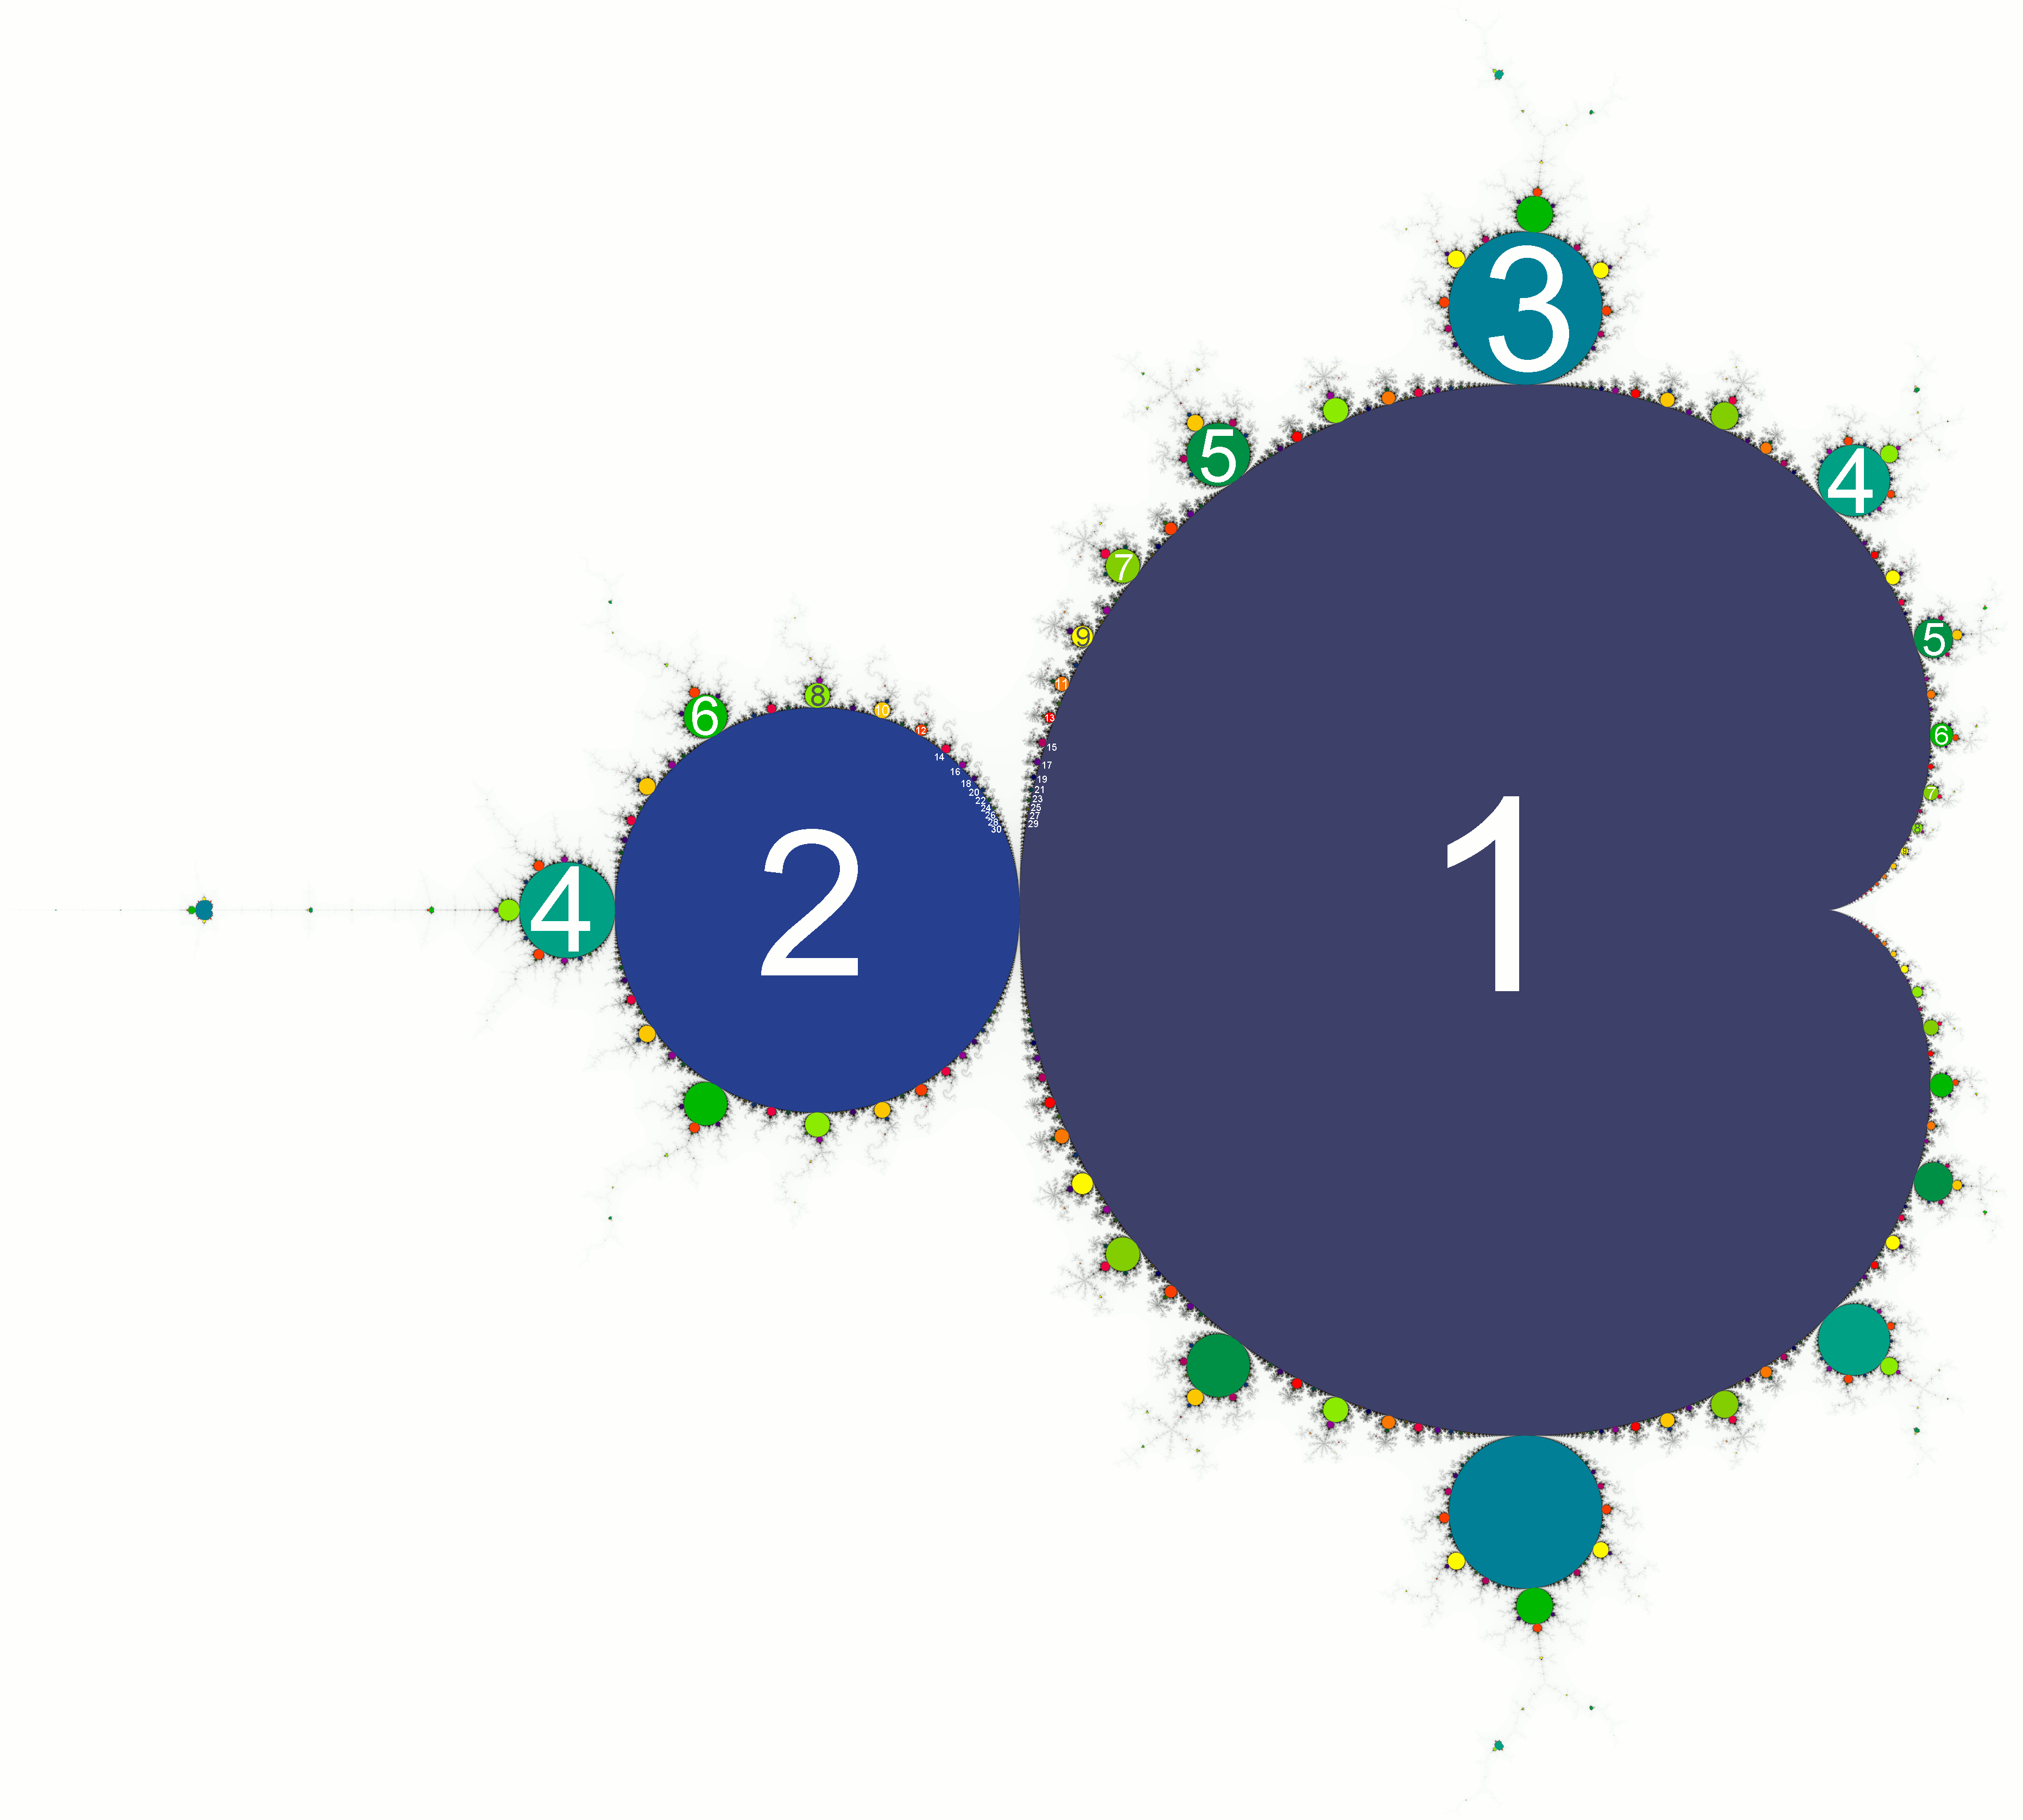
\includegraphics[width=0.62\textwidth]{bulbs.png}}
		\vspace{0.2cm}
		\captionof{figure}{Periods of hyperbolic components.} \label{fig:bulbs}
	\end{minipage}\hfill
	\begin{minipage}[b]{0.56\linewidth}
		\centering
		\scriptsize
		\begin{tabular}{|l|l|} 
			\hline
			\textbf{Optimization level} & \textbf{Execution time [s]} \\ [0.2ex] 
			\hline\hline
			\texttt{-O0} & 422.91 \\ 
			\texttt{-O1} & 230.99 \\
			\texttt{-O2} & 208.96 \\
			\texttt{-O3} & 208.49 \\
			\texttt{-O3 -ftree-vectorize} & 205.41 \\ [0.2ex] 
			\hline
		\end{tabular}
		\vspace{0.2cm}
		\caption{Execution times of \texttt{opti3} ($368.64M$ pixels, max\_iteration=$10,000$) as a function of the optimization level.}
		\label{tab:opti-levels}
		\vspace{-0.2cm}
	\end{minipage}
\end{table}
	
\end{frame}

\begin{frame}{Serial Implementations (2)}

\begin{figure}
%	\vspace{-0.7cm}
%	\centering
	\begin{subfigure}{.6\textwidth}
		\centering
		\hspace{-2cm}
		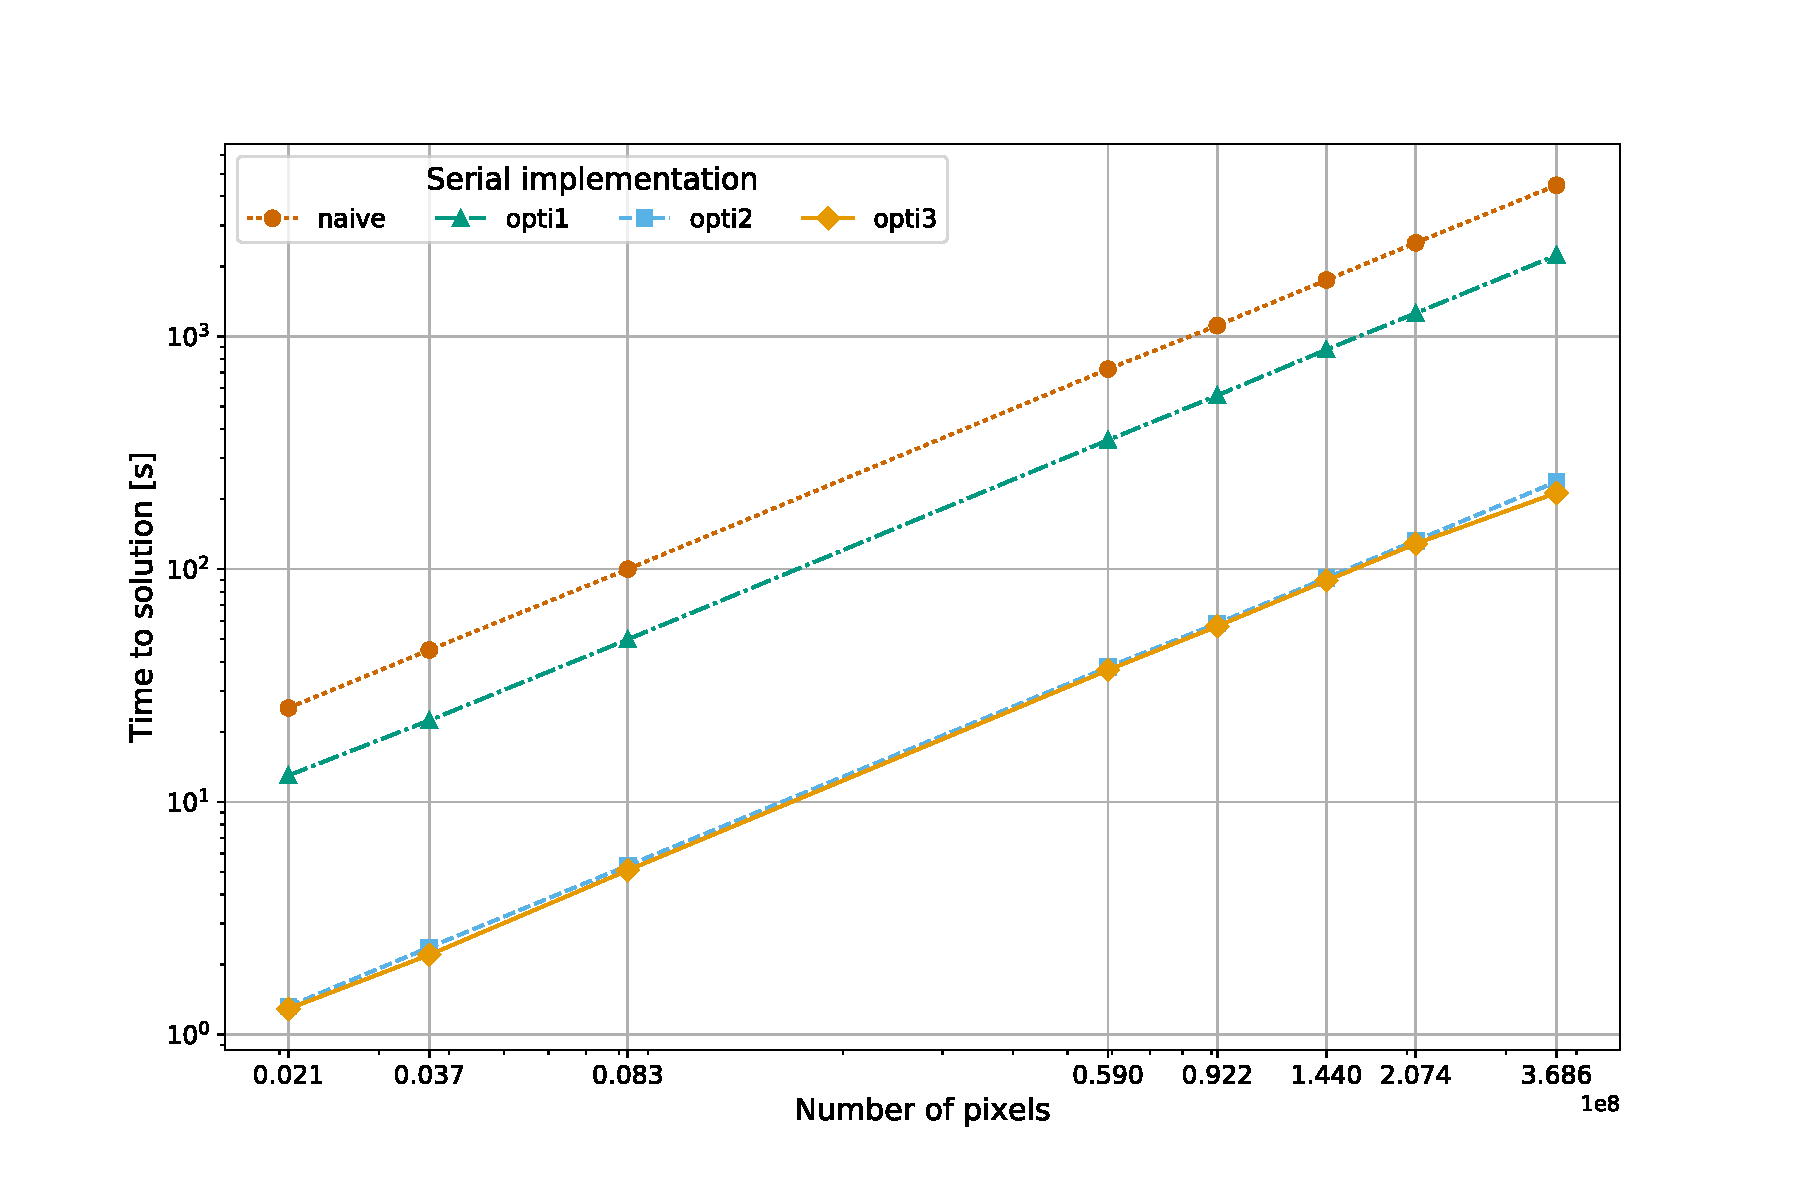
\includegraphics[width=.98\linewidth, clip, trim={1.5cm 1cm 2.5cm 2cm}]{serial-optis-px.pdf}
		\caption{} 
		\label{fig:serial-optis-px}
	\end{subfigure}%
	\begin{subfigure}{.6\textwidth}
		\centering
		\hspace{-2.5cm}
		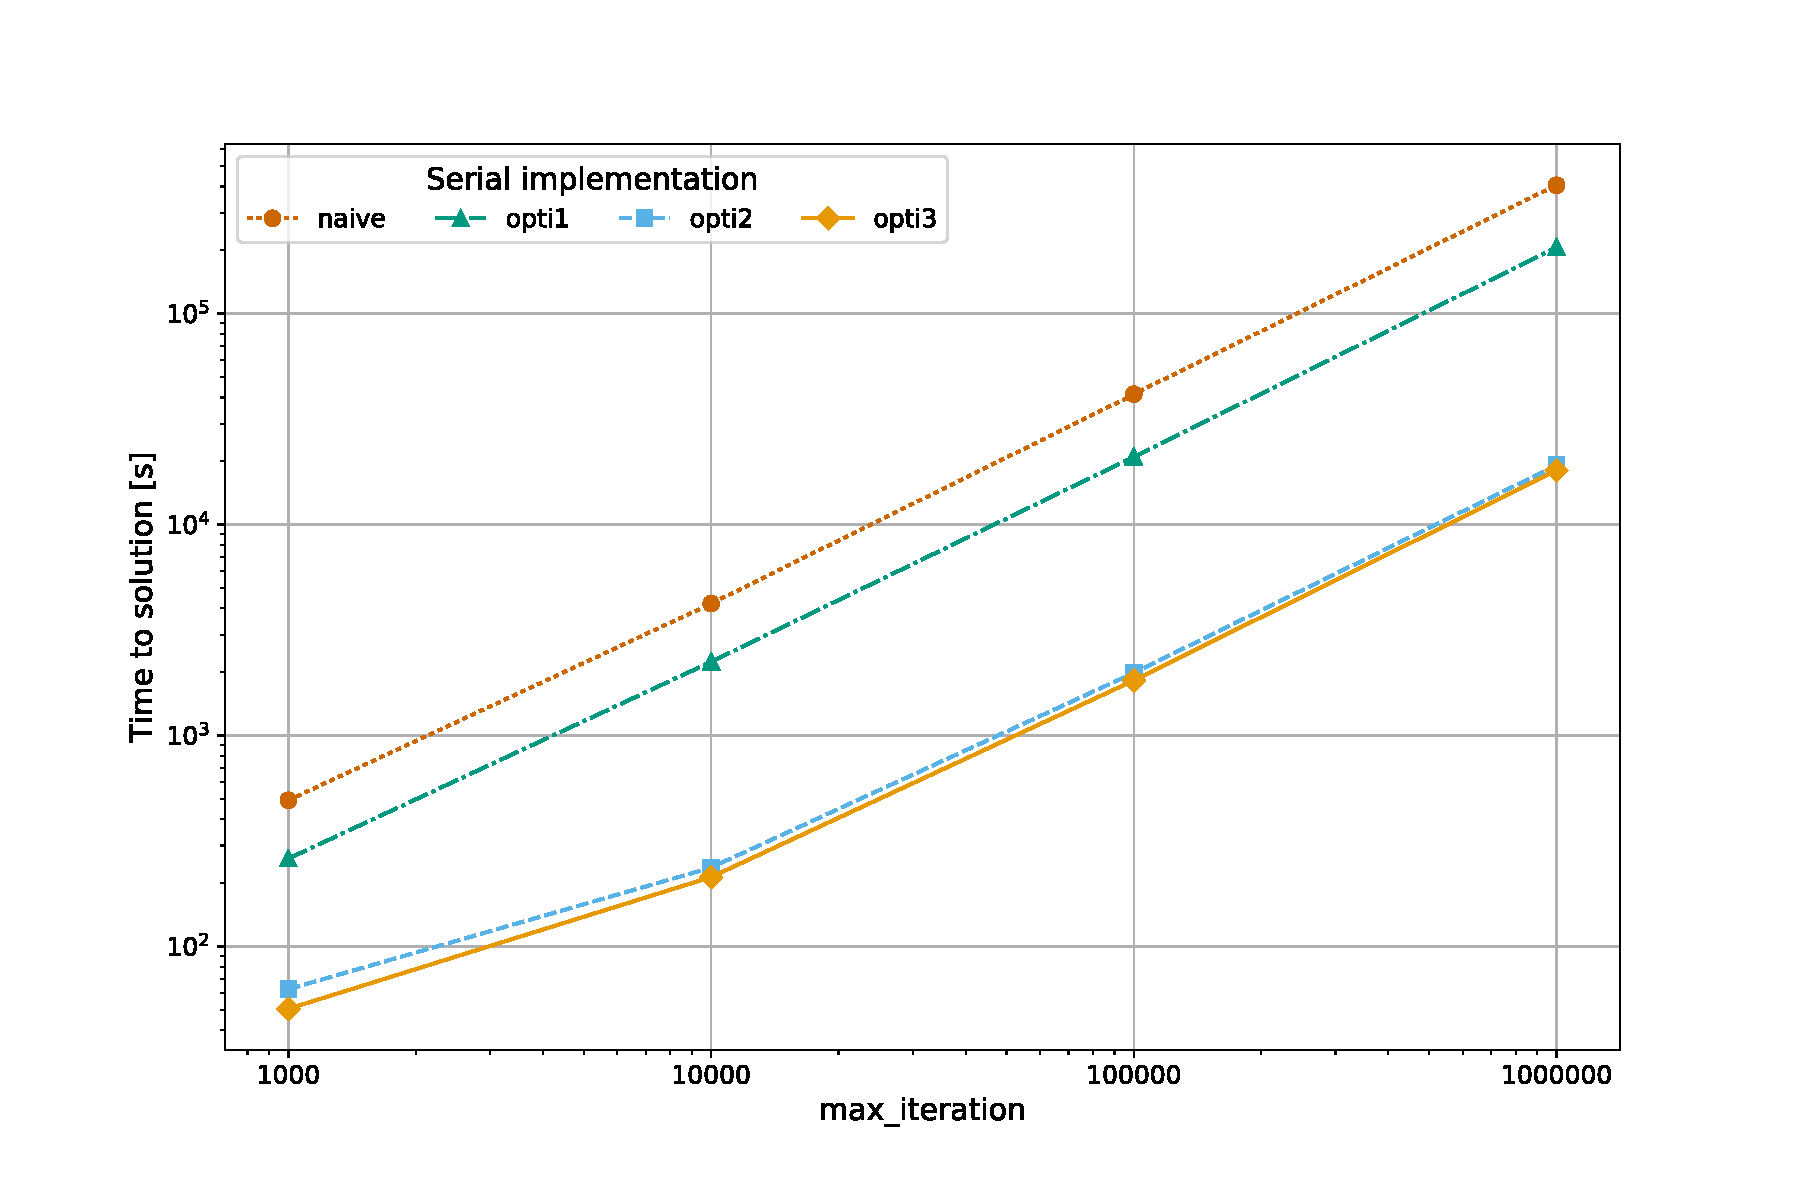
\includegraphics[width=.98\linewidth, clip, trim={1.5cm 1cm 2.5cm 2cm}]{serial-optis-maxiter.pdf}
		\caption{} 
		\label{fig:serial-optis-maxiter}
	\end{subfigure}
	\vspace{-0.4cm}
	\caption{Time to solution for the different serial implementations with respect to (a) the number of pixels (max\_iteration=10,000) and (b) max\_iteration (368,640,000 pixels).}
	\label{fig:serial-optis}
	%	\vspace{-0.2cm}
\end{figure}

\end{frame}

% -------------------------------------------------------
% -------------------------------------------------------

\section{Going Parallel}

\begin{frame}{CUDA Implementations (1)}
	
\begin{itemize}
	\item \textbf{opti3:} Parallelize escape time evaluation only.
		\begin{itemize}
			\item[$\circ$] Colors computed serially
			\item[$\circ$] $3$ matrices sent on the PCIe bus
		\end{itemize}
	\item \textbf{opti4:} All workload carried out by the GPU. 
		\begin{itemize}
			\item[$\circ$] Only exchange RGB values of the bottom part on the PCIe bus
			\item[$\circ$] Use \textit{Constant memory} to store constant values on the GPU
			\item[$\circ$] Code split into serial (\texttt{.c}) $\&$ parallel (\texttt{.cu}) parts; needs C wrapper
		\end{itemize}
	\item \textbf{opti5:} Single-precision implementation of \texttt{opti4}. 
		\begin{itemize}
			\item[$\circ$] Maximize instruction throughput
			\item[$\circ$] Cannot distinguish between double- and single-precision images
		\end{itemize}
\end{itemize}
Application profiled with \texttt{nvprof}: compute-bound.
	
\end{frame}

\begin{frame}{CUDA Implementations (2)}
	
\begin{figure}
	%	\vspace{-0.7cm}
	%	\centering
	\begin{subfigure}{.6\textwidth}
		\centering
		\hspace{-2cm}
		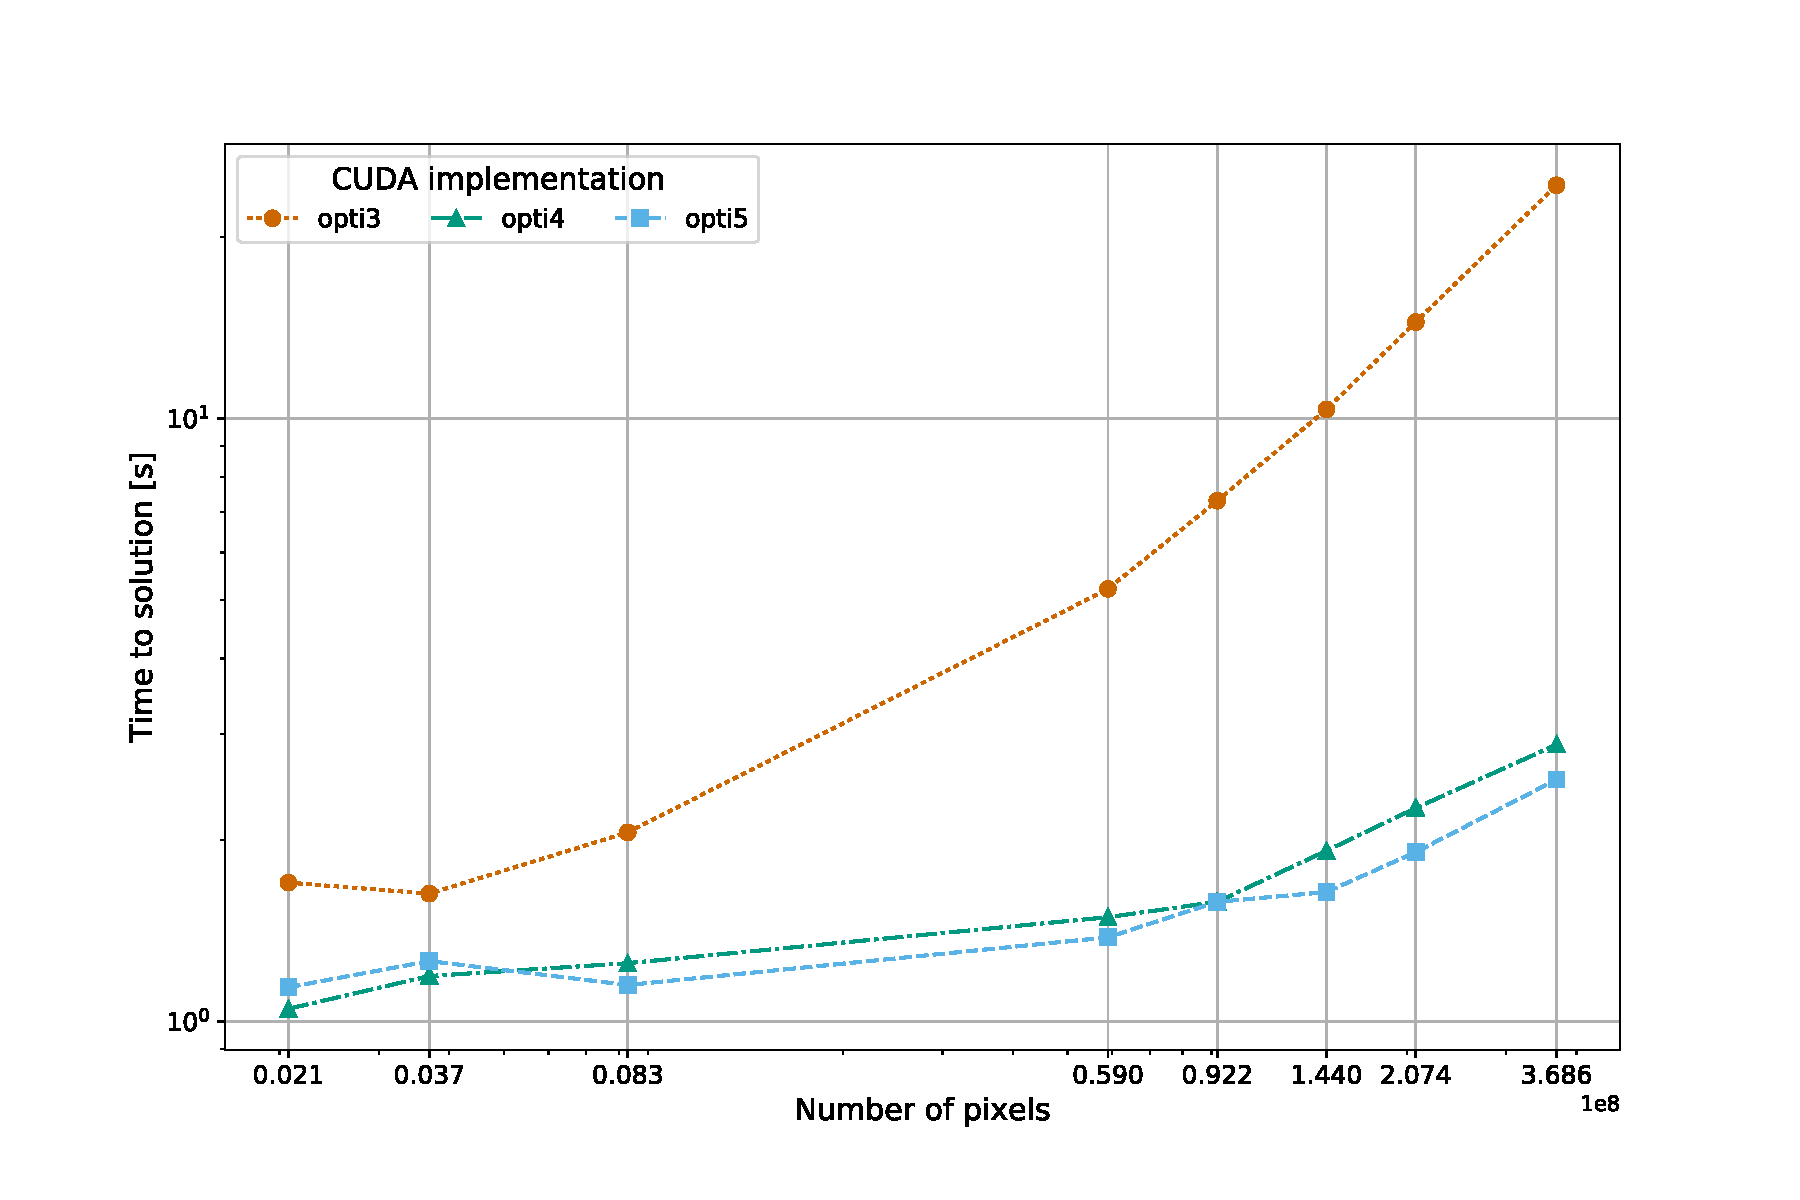
\includegraphics[width=.98\linewidth, clip, trim={1.5cm 1cm 2.5cm 2cm}]{cuda-optis-px.pdf}
		\caption{} 
		\label{fig:cuda-optis-px}
	\end{subfigure}%
	\begin{subfigure}{.6\textwidth}
		\centering
		\hspace{-2.5cm}
		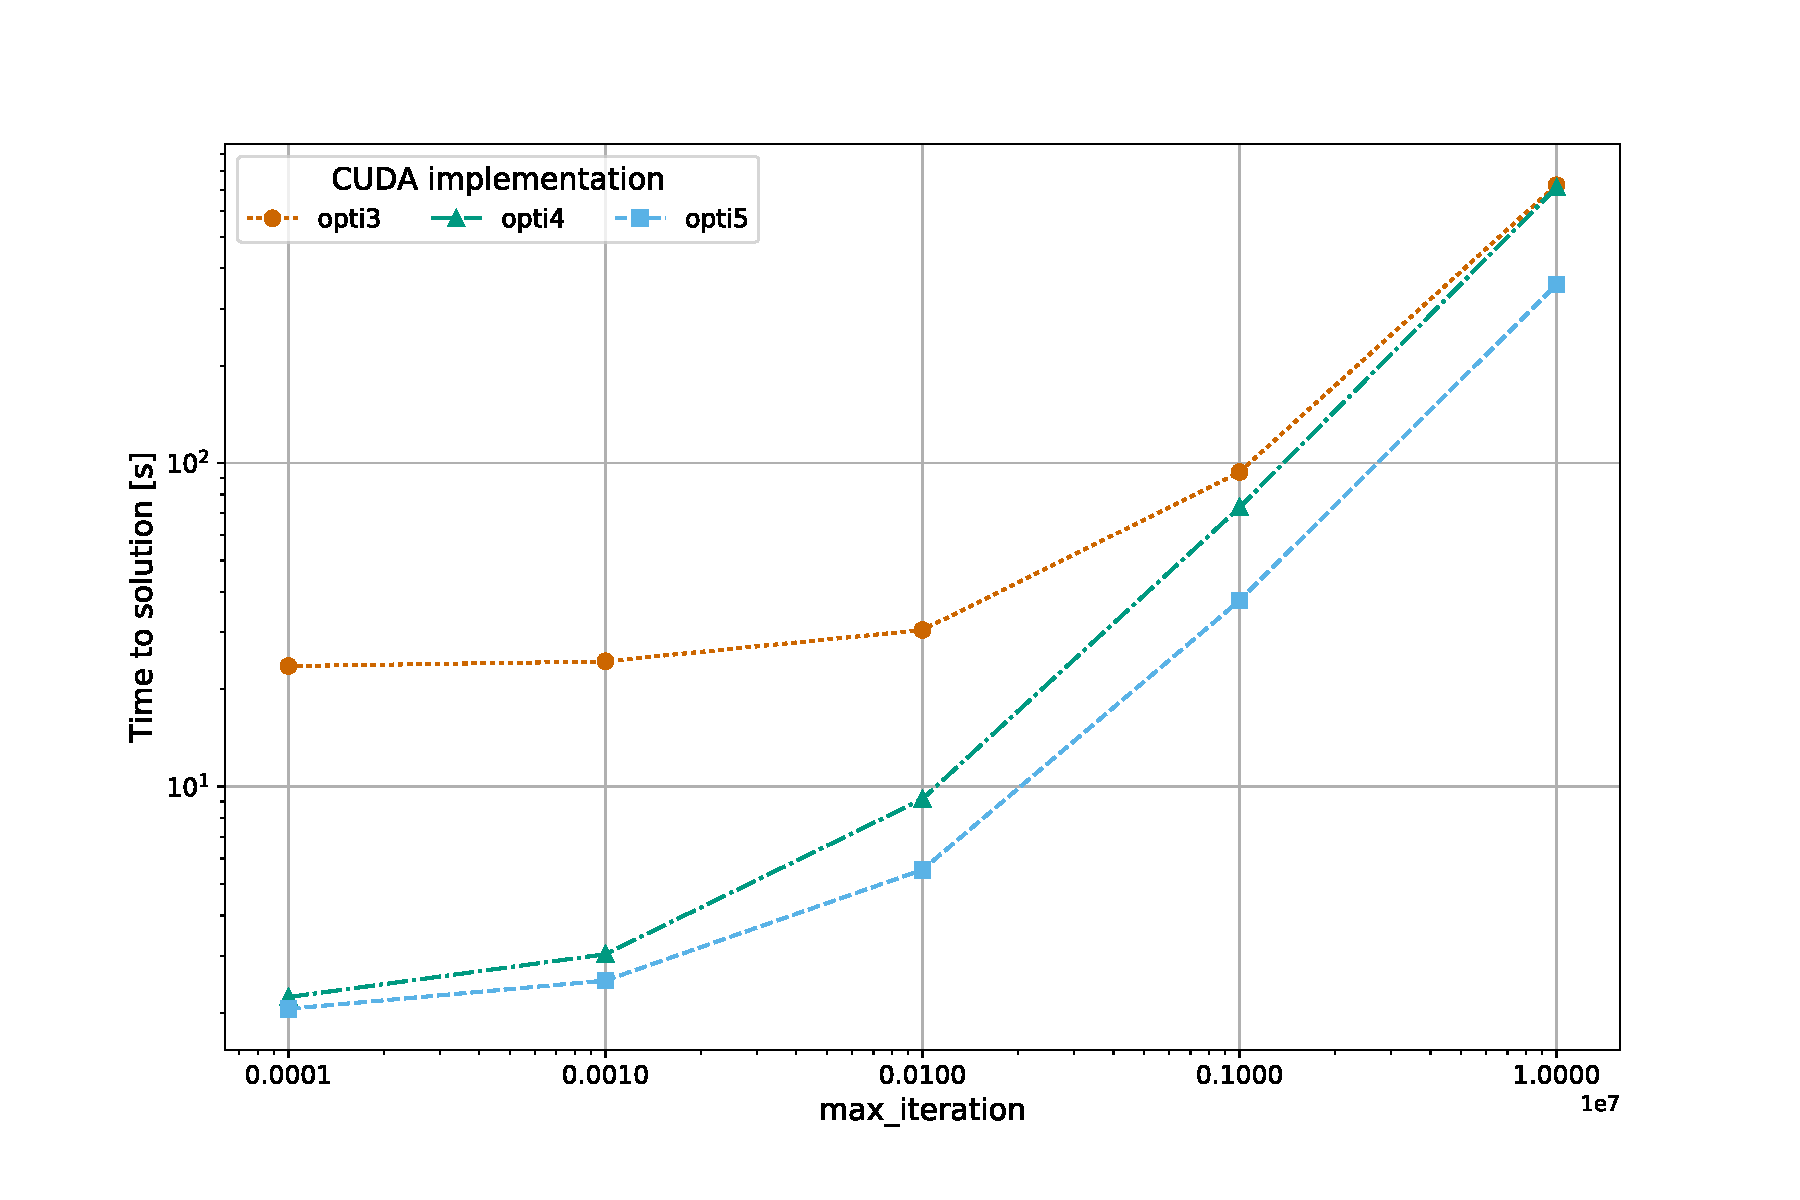
\includegraphics[width=.98\linewidth, clip, trim={1.5cm 1cm 2.5cm 2cm}]{cuda-optis-maxiter.pdf}
		\caption{} 
		\label{fig:cuda-optis-maxiter}
	\end{subfigure}
	\vspace{-0.4cm}
	\caption{Time to solution for the CUDA implementations with respect to (a) the number of pixels (max\_iteration=10,000) and (b) max\_iteration (368,640,000 pixels) with block size $512\times1$.}
	\label{fig:cuda-optis}
	%	\vspace{-0.2cm}
\end{figure}
	
\end{frame}

\begin{frame}{CUDA \textit{block size} tuning for \texttt{opti5}}

Block size: 
\begin{itemize}
	\vspace{-0.2cm}
	\item hyperparameter leading to performance improvements, increasing \textit{occupancy} $\left(\frac{active~warps}{maximum~active~warps}\right)$
	\item It depends on both the problem and the specifics of the GPU
\end{itemize}

\begin{table}[H]
	\vspace{-0.1cm}
	\footnotesize
	\hspace{-1.8cm}
	\begin{subtable}{.38\linewidth}
		\centering
		\begin{tabular}{|l|l|l|} 
			\hline
			\textbf{Block size} & \multicolumn{2}{|c|}{\textbf{Occupancy [$\%$]}} \\
			\cline{2-3}
			& \texttt{2560x1440} & \texttt{25600x14400} \\ [0.2ex] 
			\hline\hline
			\texttt{32x1} & 18.05 & 18.81 \\ 
			\texttt{64x1} & 25.41 & 32.65 \\
			\texttt{128x1} & 31.82 & 51.52 \\
			% \texttt{192x1} & 34.85 & 56.01 \\
			\texttt{256x1} & \textbf{36.15} & \textbf{58.80} \\
			% \texttt{384x1} & 35.62 & 57.30 \\
			\texttt{512x1} & 28.76 & 52.37 \\
			%			\texttt{768x1} & 13.79 & 37.59 \\
			\texttt{1024x1} & 8.39 & 25.50 \\
			\texttt{8x8} & 19.04 & 20.12 \\
			\texttt{16x16} & 26.91 & 25.93 \\
			\texttt{32x32} & 5.91 & 7.74 \\ [0.2ex] 
			\hline
		\end{tabular}
	\end{subtable}%
	\hspace{1.8cm}
	\begin{subtable}{.38\linewidth}
		\centering
		\begin{tabular}{|l|l|l|} 
			\hline
			\textbf{Block size} & \multicolumn{2}{|c|}{\textbf{Execution time [s]}} \\
			\cline{2-3}
			& \texttt{2560x1440} & \texttt{25600x14400} \\ [0.2ex] 
			\hline\hline
			\texttt{32x1} & 2.53 & 79.61 \\ 
			\texttt{64x1} & 2.29 & 50.32 \\
			\texttt{128x1} & 2.10 & 37.52 \\
			% \texttt{192x1} & 2.05 & 36.56 \\
			\texttt{256x1} & \textbf{2.04} & \textbf{35.91} \\
			% \texttt{384x1} & 2.11 & 36.60 \\
			\texttt{512x1} & 2.17 & 37.69 \\
			%			\texttt{768x1} & 2.38 & 44.73 \\
			\texttt{1024x1} & 5.65 & 90.60 \\
			\texttt{8x8} & 4.09 & 237.72 \\
			\texttt{16x16} & 2.45 & 97.12 \\
			\texttt{32x32} & 7.48 & 270.24 \\ [0.2ex] 
			\hline
		\end{tabular}
	\end{subtable} 
	\caption{Occupancy and execution time for two image sizes as the block size varies for max\_iteration=$10,000$. Evaluated using \texttt{nvprof}.}
\end{table}

\end{frame}

\begin{frame}{Hybrid Implementations (1)}
	
	Distribute the computations over different CPUs and GPUs with \texttt{MPI}.
	\begin{itemize}
		\item Image split to the $2$ processors in a node, each uses $1$ GPU.
		\begin{itemize}
			\item[$\circ$] Non-blocking, point-to-point communications where rank $0$-processor receives the image parts out-of-order~\footnote{No \texttt{MPI\_Barrier()} used.\label{no_barrier}}
			\item[$\circ$] Parallel I/O
		\end{itemize}	
		\item Image split to the $2$ processors in a node, each uses $2$ GPUs.\\
		Highest performance: all the CUDA functions are asynchronous~\footnote{No \texttt{\_\_syncthreads()} used.}
		\begin{itemize}
			\vspace{-0.5cm}
			\item[$\circ$] Non-blocking, point-to-point communications where rank $0$-processor receives the image parts out-of-order~\textsuperscript{\ref{no_barrier}}
			\item[$\circ$] Parallel I/O
		\end{itemize}
		\begin{figure}
%			\vspace{-0.4cm}
%			\hspace{2.5cm}
			\centering
			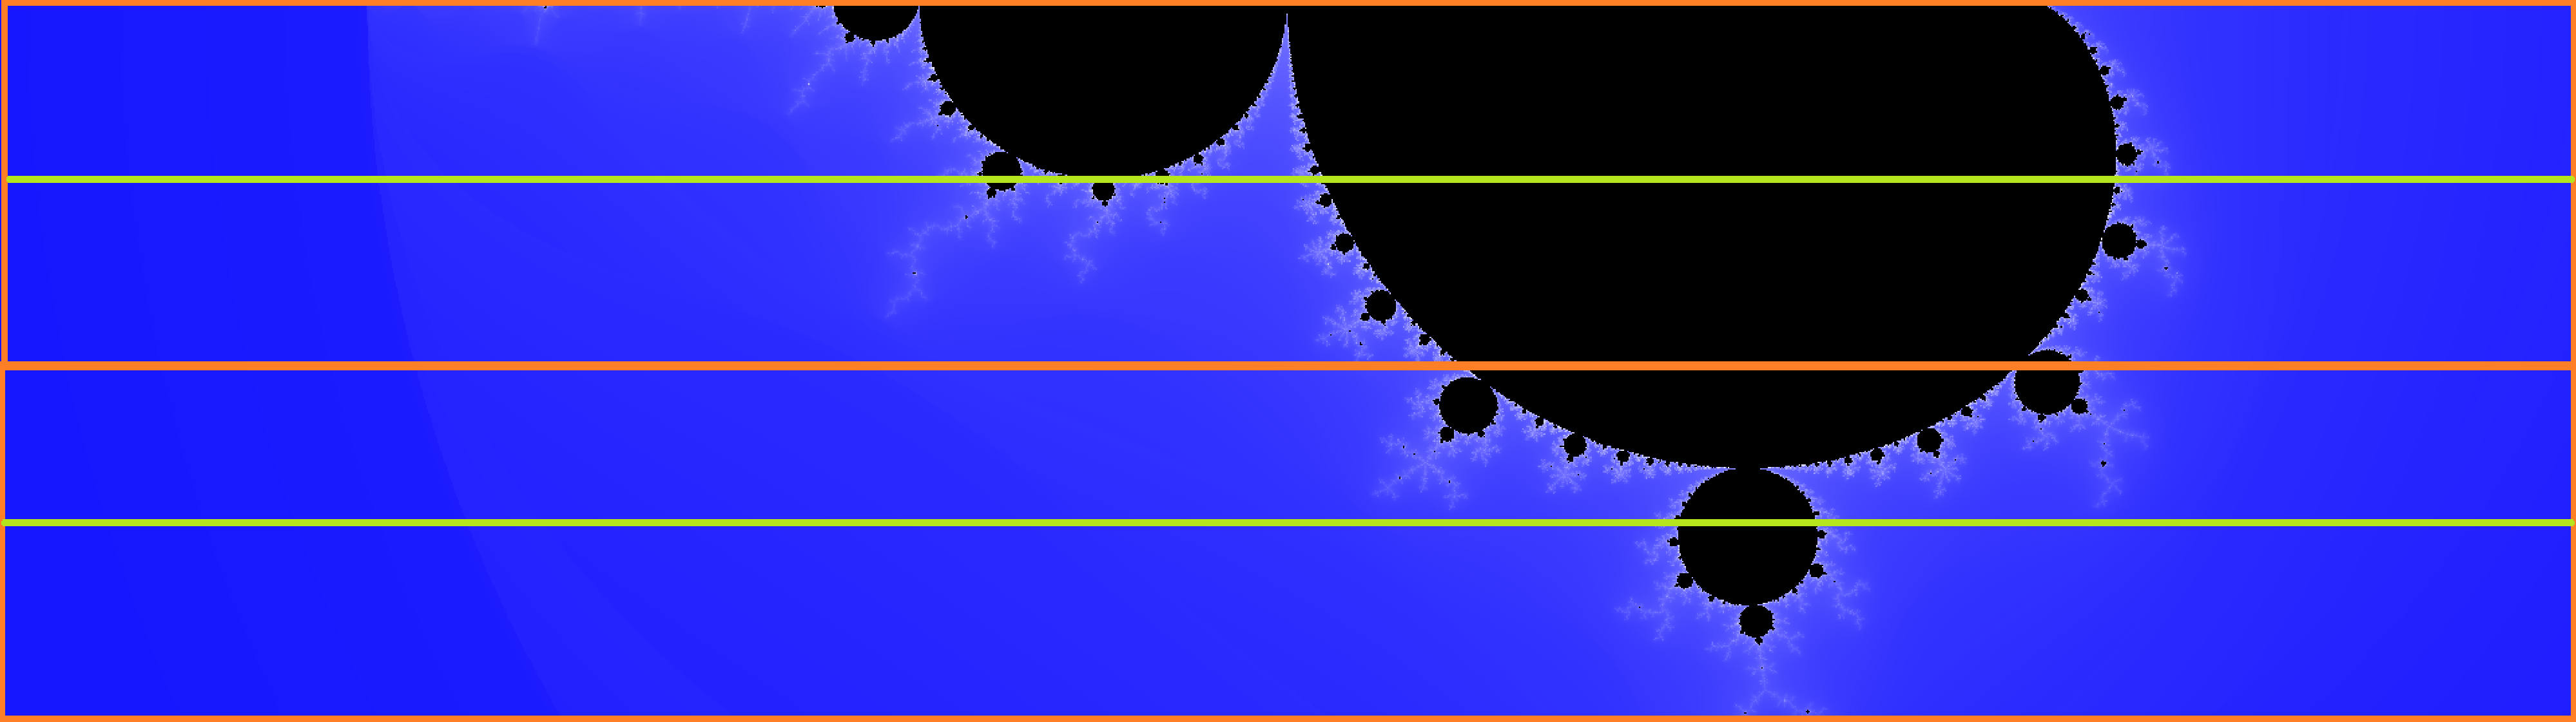
\includegraphics[width=.7\linewidth]{hybrid-split.pdf}
			\vspace{-0.2cm}
			\caption{Image split to CPUs (orange) and GPUs (orange or green).}
			\label{fig:hybrid-split}
		\end{figure}
		
	\end{itemize}

\end{frame}

\begin{frame}{Hybrid Implementations (2)}
	
	\begin{figure}
		%	\vspace{-0.7cm}
		%	\centering
		\begin{subfigure}{.6\textwidth}
			\centering
			\hspace{-2cm}
			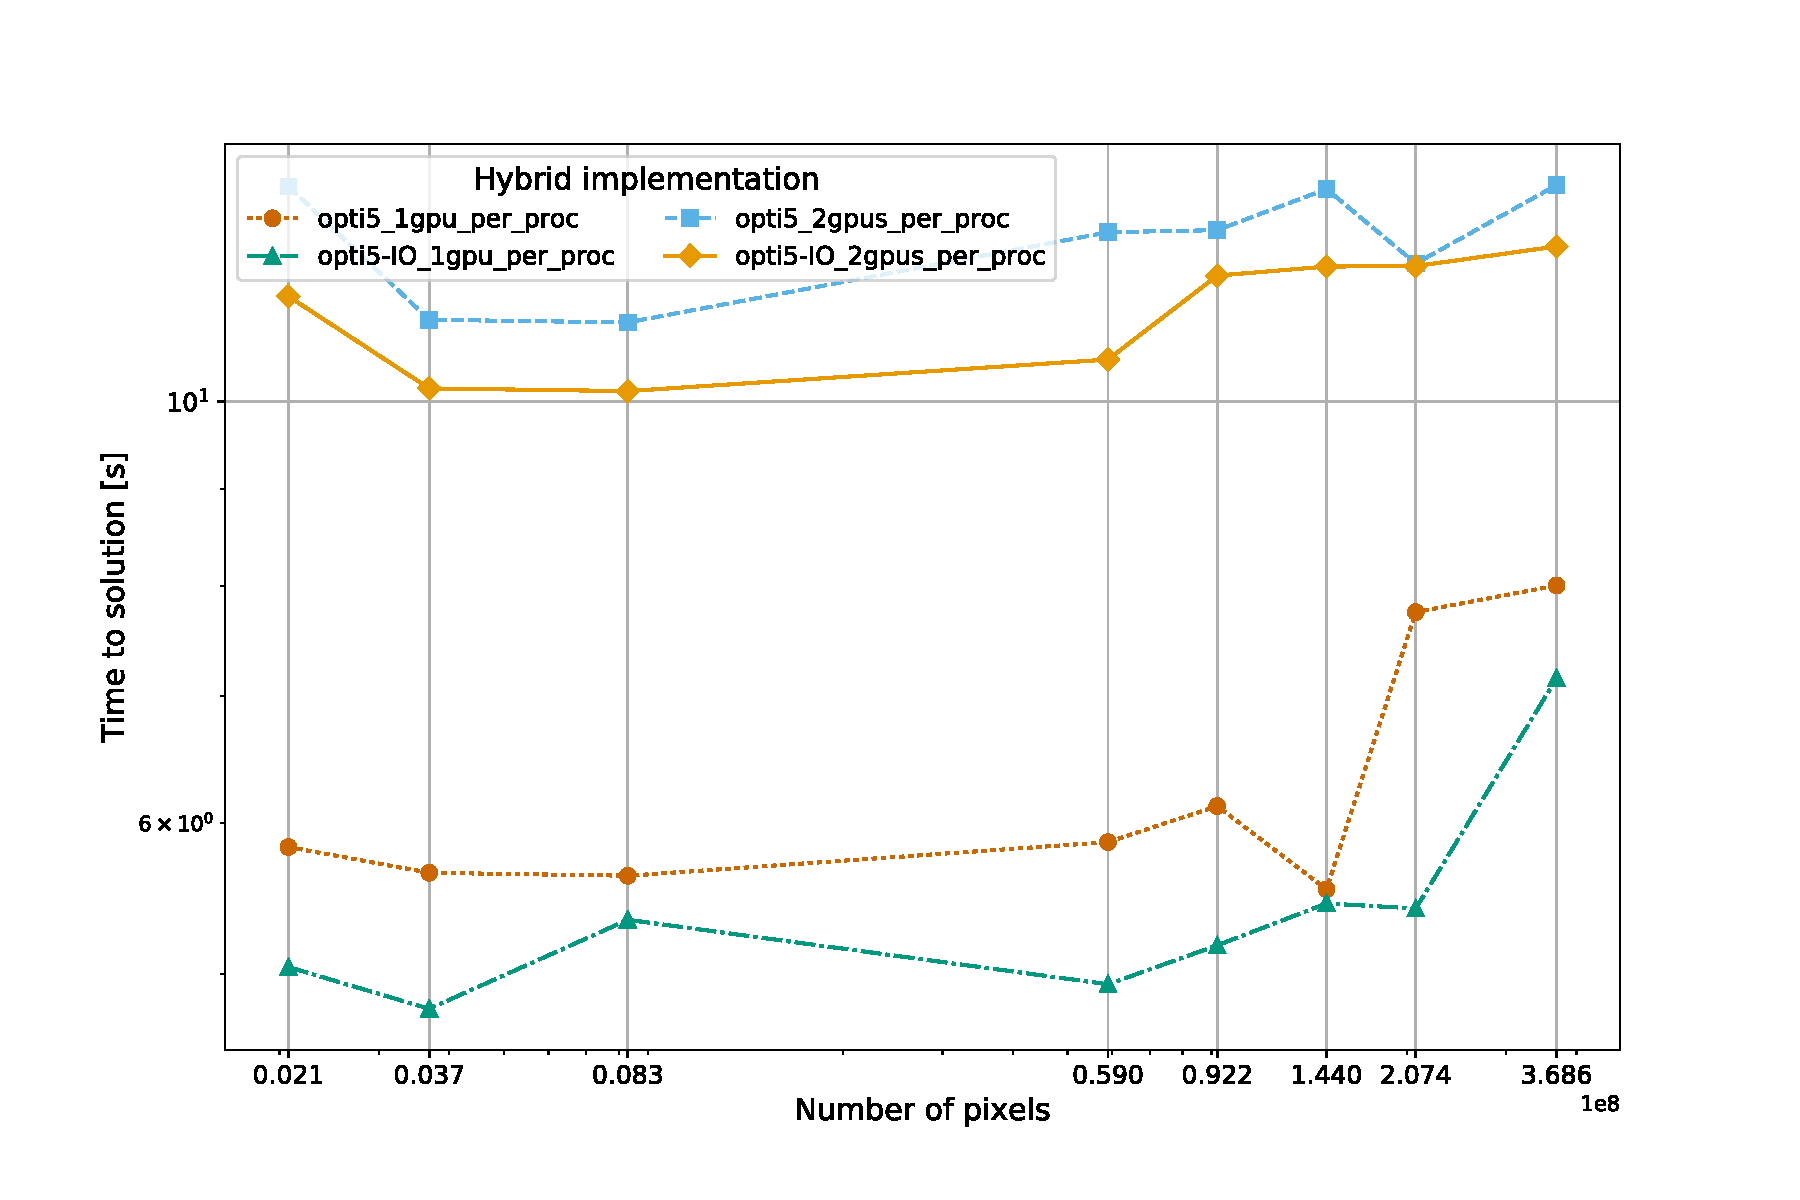
\includegraphics[width=.98\linewidth, clip, trim={1.5cm 1cm 2.5cm 2cm}]{hybrid-optis-px.pdf}
			\caption{} 
			\label{fig:hybrid-optis-px}
		\end{subfigure}%
		\begin{subfigure}{.6\textwidth}
			\centering
			\hspace{-2.5cm}
			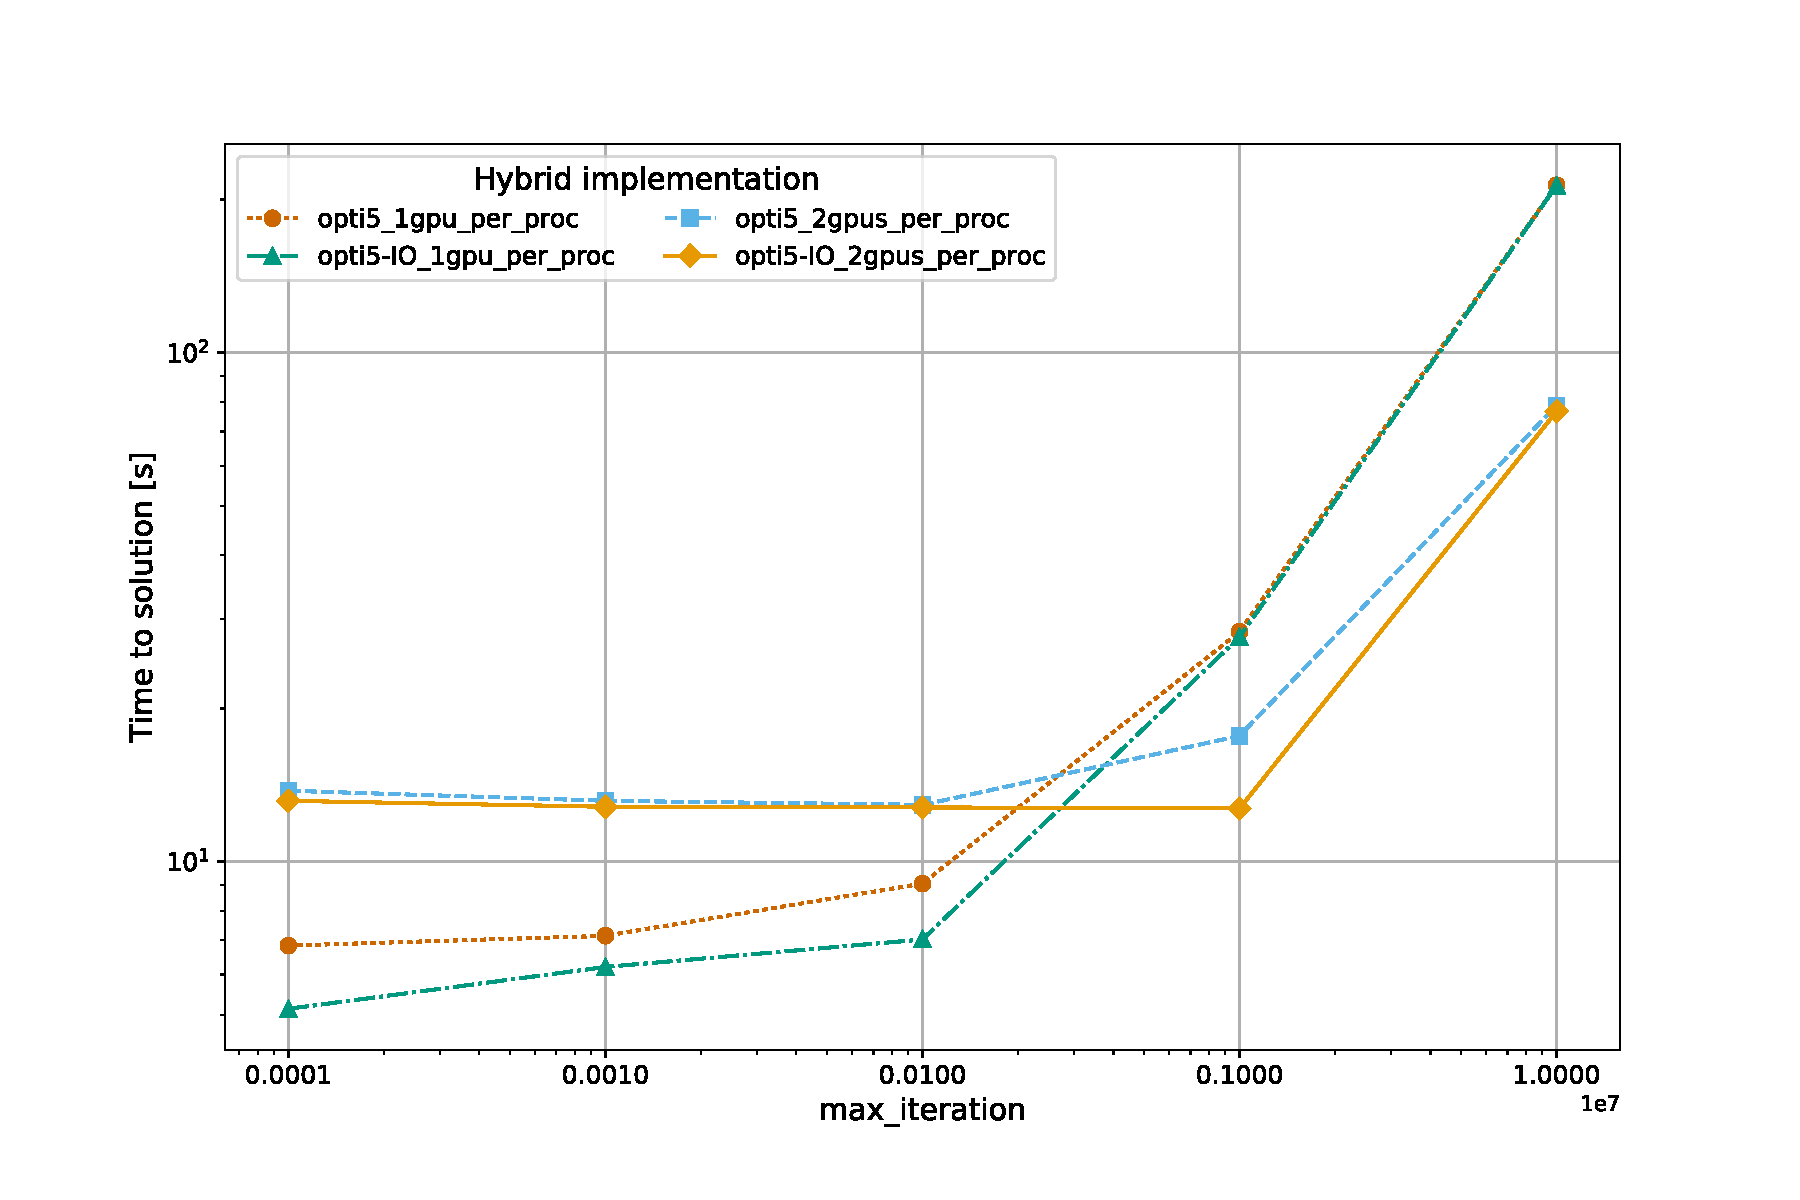
\includegraphics[width=.98\linewidth, clip, trim={1.5cm 1cm 2.5cm 2cm}]{hybrid-optis-maxiter.pdf}
			\caption{} 
			\label{fig:hybrid-optis-maxiter}
		\end{subfigure}
		\vspace{-0.4cm}
		\caption{Time to solution for the hybrid implementations with respect to (a) the number of pixels (max\_iteration=10,000) and (b) max\_iteration (368,640,000 pixels) with block size $256\times1$.}
		\label{fig:hybrid-optis}
		%	\vspace{-0.2cm}
	\end{figure}
	
\end{frame}


% -------------------------------------------------------
% -------------------------------------------------------

\section{Results}

\begin{frame}{Strong Scaling}
	
	\begin{figure}
		%	\vspace{-0.7cm}
		%	\centering
		\begin{subfigure}{.6\textwidth}
			\centering
			\hspace{-2cm}
			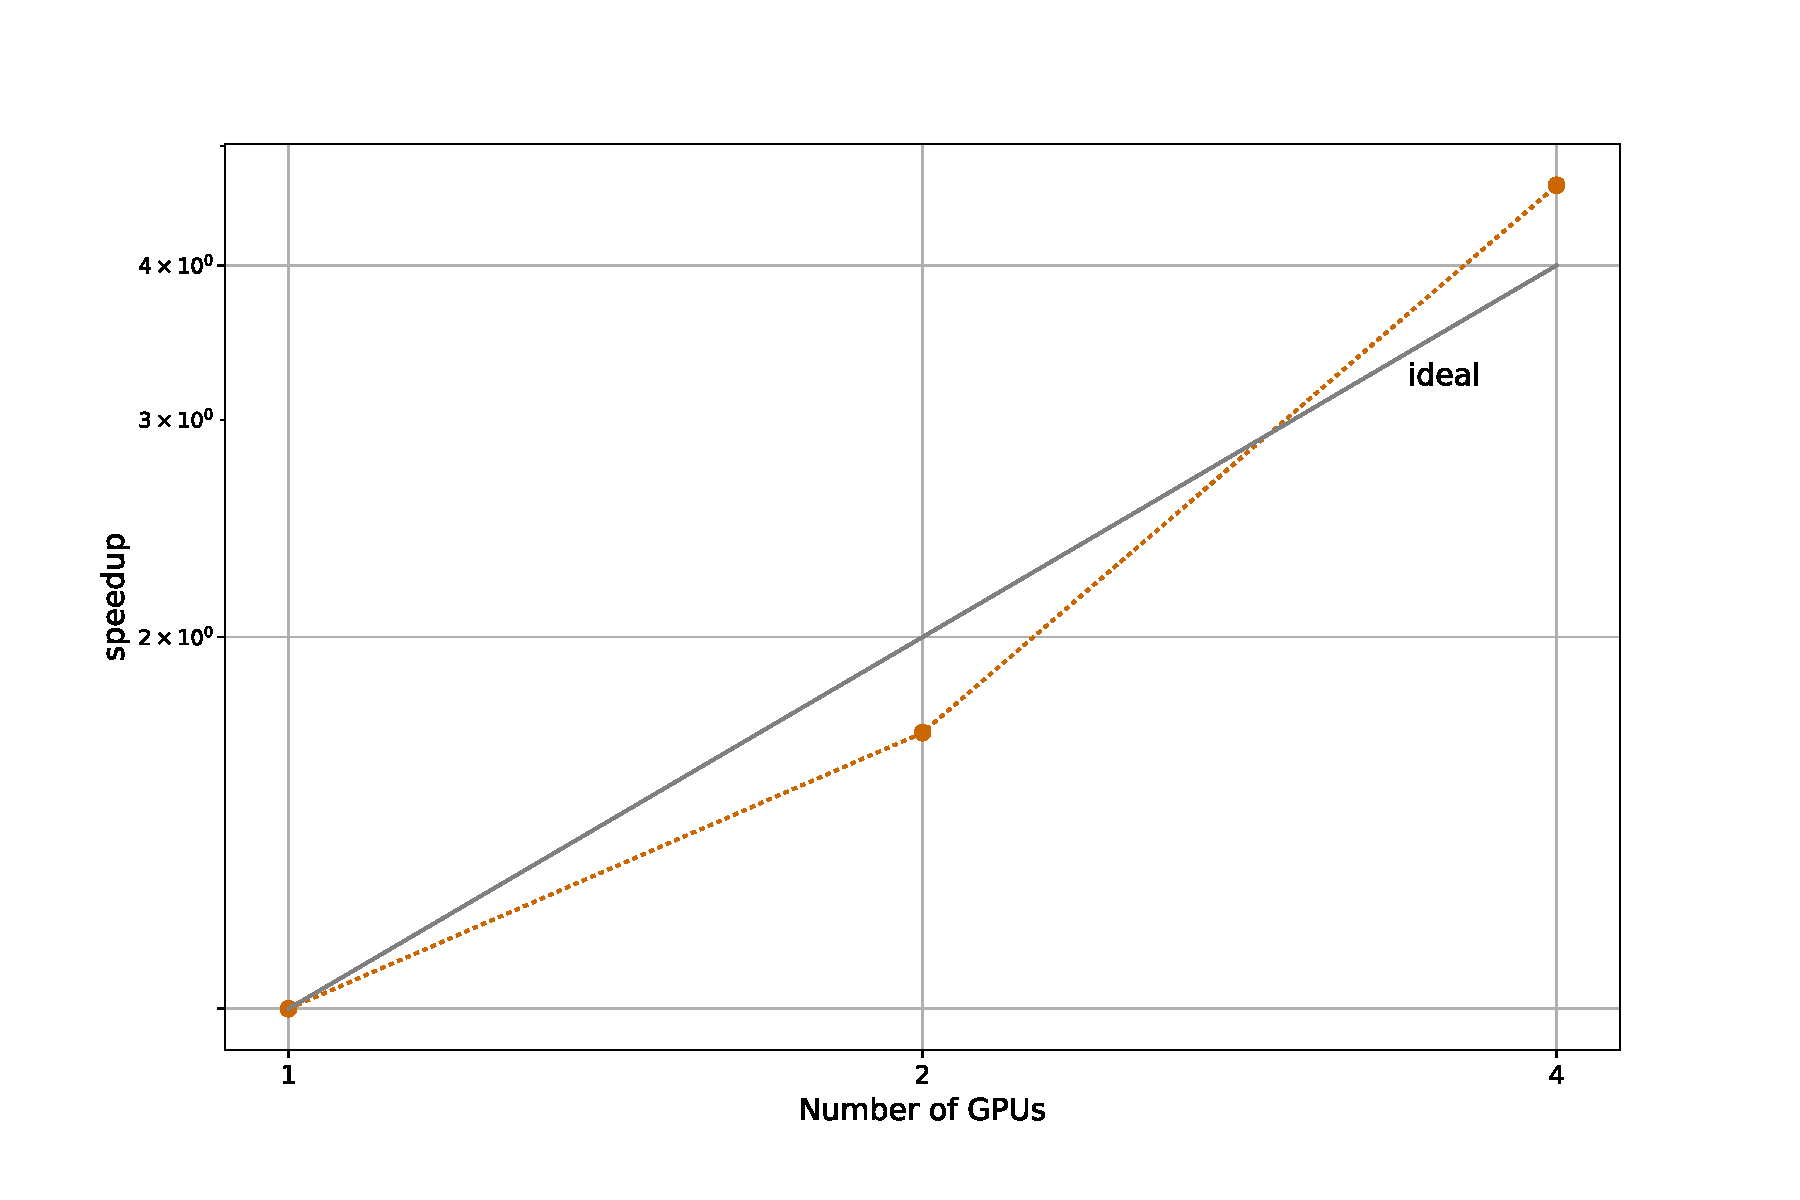
\includegraphics[width=.98\linewidth, clip, trim={1.5cm 1cm 2.5cm 2cm}]{strong-mpi.pdf}
%			\vspace{-0.2cm}
			\caption{} 
			\label{fig:strong-mpi}
		\end{subfigure}%
		\begin{subfigure}{.6\textwidth}
			\centering
			\hspace{-2.5cm}
			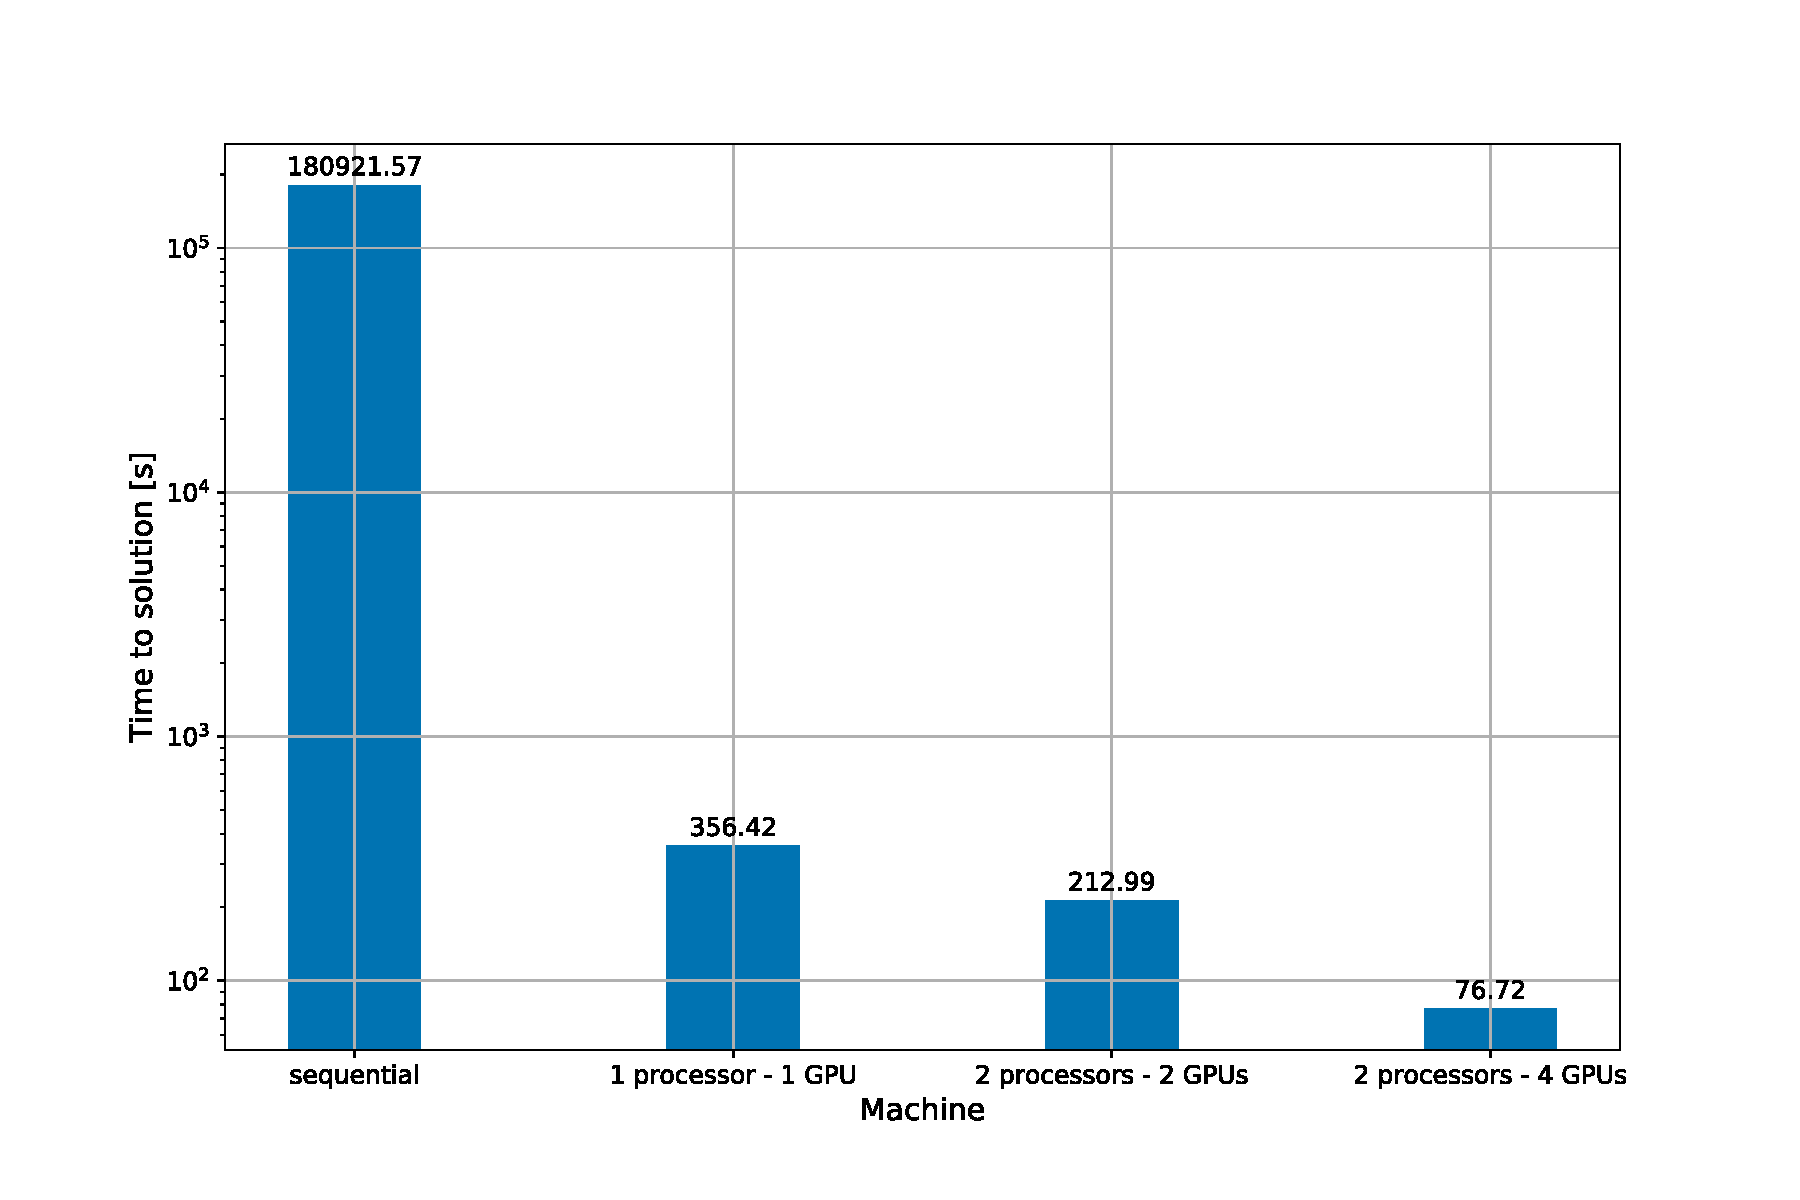
\includegraphics[width=.98\linewidth, clip, trim={1.5cm 1cm 2.5cm 2cm}]{strong-tts.pdf}
%			\vspace{-0.2cm}
			\caption{} 
			\label{fig:strong-tts}
		\end{subfigure}
		\vspace{-0.4cm}
		\caption{Strong scaling as (a) the speedup for an increasing number of GPUs (via \texttt{MPI}) and (b) the reduced time to solution of the same problem ($368.64M$-pixel image, max\_iteration=$10\times10^6$) for the different versions.}
		\label{fig:strong}
%		\vspace{-0.4cm}
	\end{figure}
		
\end{frame}

\begin{frame}{Weak Scaling}
	
	\begin{figure}
		%	\vspace{-0.7cm}
		\centering
		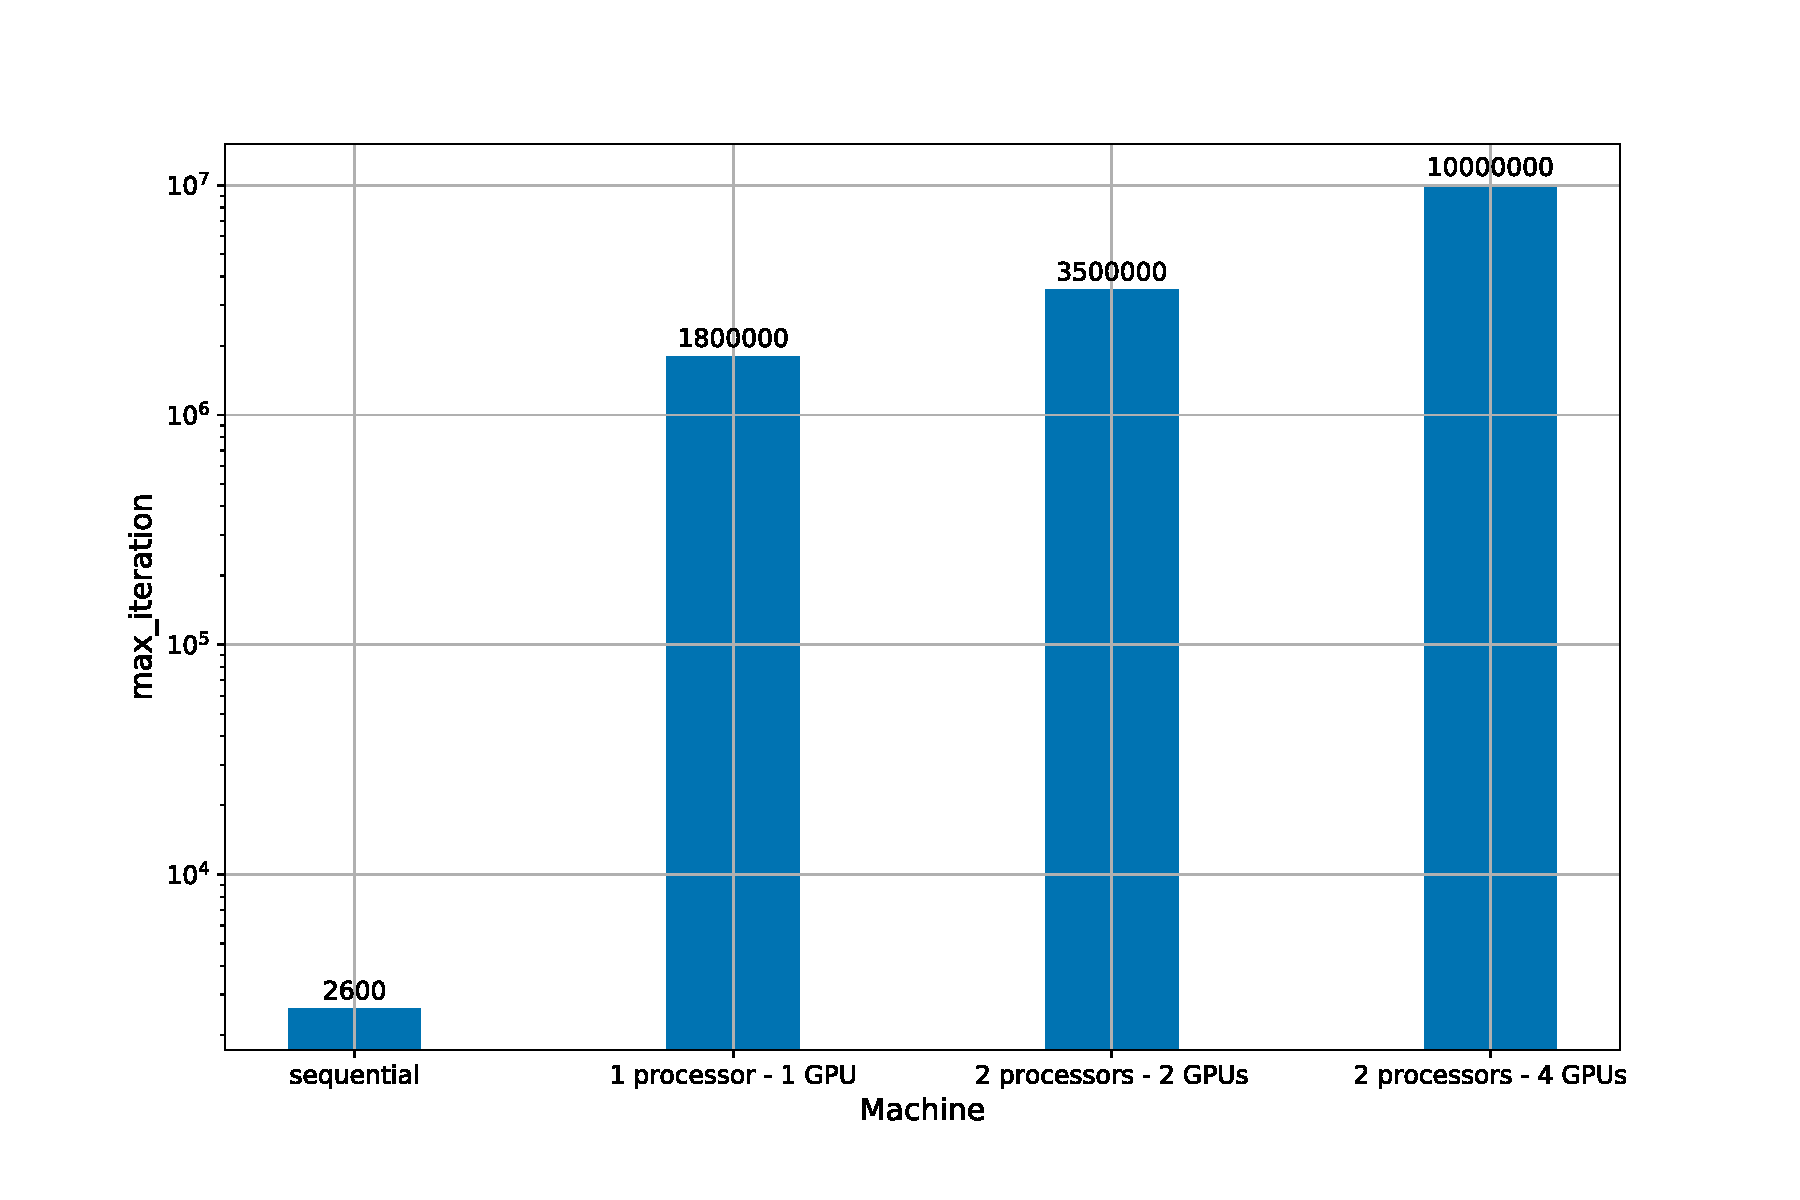
\includegraphics[width = 0.8\textwidth, clip, trim={1.5cm 1cm 2cm 2cm}]{weak.pdf}
		\caption{Weak scaling as a function of the problem size that can be solved in the same amount of time ($76~s$) by the different versions.}
		\label{fig:weak}
		%		\vspace{-0.4cm}
	\end{figure}
	
\end{frame}


% -------------------------------------------------------
% -------------------------------------------------------

\section{Conclusion}

\begin{frame}{Conclusion \& Future Work}
\textbf{Conclusion}
\begin{itemize}
	\vspace{-0.2cm}
	\item Implement and optimize \texttt{serial}, \texttt{CUDA} and \texttt{CUDA+MPI} applications
	\item Gain experience with \texttt{CUDA} and \texttt{MPI} in a supercomputer
	\item Acquire familiarity with profiling tools
	\item Investigate different technologies
	\begin{itemize}
		\item[$\circ$] Non-blocking communications and parallel I/O in \texttt{MPI}
		\item[$\circ$] Asynchronous functions in \texttt{CUDA}
	\end{itemize}
\end{itemize}

\textbf{Future Work}
\begin{itemize}
	\vspace{-0.2cm}
	\item Experiment with 2D grids
	\item Investigate the impact of external libraries
	\item Explore different algorithms
\end{itemize}
% errors -- bugs
% \vfill
\pause
%\begin{tcolorbox}
\fontfamily{qzc}\selectfont % TeX Gyre Schola (similar to Zapf Chancery)
\hfill
\huge
%\tcbox{
\alert{Thank you}
%\end{tcolorbox}

\end{frame}


\end{document}
